\documentclass[12pt,a4paper]{article}

\usepackage[ngerman]{babel}
\usepackage[T1]{fontenc}
\usepackage[utf8]{inputenc}
\usepackage{amsmath,amssymb}
\usepackage{geometry}
\usepackage{setspace}
\usepackage{hyperref}
\usepackage{graphicx}

\geometry{margin=2.5cm}
\onehalfspacing

\title{Kapitel 5 -- Ergebnisse}
\author{}
\date{}

\begin{document}
\maketitle

\section{Ergebnisse}

\subsection{Topologische Eigenschaften der untersuchten Netzwerke}

Bevor die Robustheit der Netzwerke unter Störungen analysiert wird, ist es
sinnvoll, die grundlegenden topologischen Eigenschaften der betrachteten
Netzwerke zu vergleichen. Diese Eigenschaften bestimmen maßgeblich, wie ein
Netzwerk auf Knotenentfernungen reagiert. Die Analyse bezieht sich auf den
Ausgangszustand der Netzwerke ohne Knotenentfernung ($q = 0$), der in den
Simulationsdaten explizit enthalten ist.\\
Untersucht werden drei synthetische Netzwerkmodelle: ein Erdős--Rényi-Zufallsgraph
(ER), ein Watts--Strogatz-Small-World-Netzwerk (WS) und ein
Barabási--Albert-Netzwerk (BA). Alle Netzwerke besitzen dieselbe Knotenzahl
($n=800$), wodurch strukturelle Unterschiede direkt vergleichbar sind.

\paragraph{Gradstruktur und Vernetzung}
Die drei Modelle unterscheiden sich deutlich in ihrer Gradstruktur. Der
Erdős--Rényi-Graph weist eine relativ homogene Gradverteilung auf: die meisten
Knoten besitzen einen ähnlichen Grad, extreme Abweichungen sind selten. Das
Watts--Strogatz-Netzwerk ist ebenfalls vergleichsweise homogen, besitzt aber
durch seine Ausgangsringstruktur eine deutlich stärkere lokale Vernetzung. Beim
Barabási--Albert-Netzwerk ist die Gradverteilung stark heterogen: wenige Knoten
fungieren als Hubs mit sehr hohem Grad, während der Großteil nur schwach
vernetzt ist. Diese Hub-Struktur ist für skalenfreie Netze typisch und wirkt
sich später stark auf die Robustheit unter gezielten Angriffen aus.

\paragraph{Clustering und lokale Struktur}
Ein zentraler Unterschied zeigt sich im Clustering. Das Watts--Strogatz-Netzwerk
besitzt sowohl einen hohen globalen Clustering-Wert als auch hohe mittlere
lokale Clustering-Koeffizienten. Das bestätigt die typische Small-World-Logik:
lokal dicht, global trotzdem kurze Wege. Der Erdős--Rényi-Graph hat dagegen nur
geringe Clustering-Werte; lokale Dreiecke entstehen hier eher zufällig. Das
Barabási--Albert-Netzwerk liegt dazwischen: es kann lokal durchaus Clustering
zeigen, jedoch ungleich verteilt (oft stärker um zentrale Knoten herum).

\paragraph{Pfadlängen und Durchmesser}
Mittlere kürzeste Pfadlänge und Durchmesser geben einen Eindruck der globalen
Erreichbarkeit. Erdős--Rényi und Watts--Strogatz zeigen im Ausgangszustand kurze
mittlere Pfadlängen. Beim Watts--Strogatz-Modell ist interessant, dass diese
kurzen Wege trotz hoher lokaler Struktur entstehen. Das Barabási--Albert-Netz
weist ebenfalls kurze Pfadlängen auf, was vor allem an den Hubs liegt, über die
viele kürzeste Wege laufen. Der Durchmesser ist dabei ein empfindlicherer
Indikator: er bleibt oft moderat, kann aber bei strukturellen Eingriffen schnell
ansteigen, wenn zentrale Vermittlerknoten verloren gehen.

\paragraph{Einordnung für die Robustheitsanalyse}
Diese topologischen Unterschiede bilden die Ausgangslage für die folgenden
Robustheitsanalysen. Homogene Gradverteilungen (ER, teilweise WS) sprechen für
eine gleichmäßigere Reaktion auf zufällige Ausfälle. Hohe lokale Clusterbildung
(WS) deutet auf Redundanz im Nahbereich hin. Die Hub-Struktur (BA) lässt
hingegen eine starke Robustheit bei Random Failures, aber eine hohe
Verwundbarkeit bei gezielten Angriffen erwarten. Ob und wie deutlich sich das
in den Simulationen zeigt, wird in den nächsten Unterabschnitten mit
Robustheitskurven und AUC-Kennzahlen überprüft.

\subsection{Robustheit unter zufälligen Ausfällen}

In diesem Abschnitt wird das Robustheitsverhalten der untersuchten
Netzwerkmodelle unter zufälligen Knotenausfällen analysiert. Zufällige Ausfälle
modellieren Störungen ohne gezielte Auswahl einzelner Knoten, wie sie etwa durch
technische Defekte oder lokale externe Einwirkungen auftreten können. Zur
Bewertung wird die Konnektivität der verbleibenden Netzwerke in Abhängigkeit vom
Anteil entfernter Knoten betrachtet.\\
Als zentrale Metrik wird die Größe der größten verbundenen Komponente relativ zur
Anzahl der verbleibenden Knoten verwendet,
\[
S_{\text{surv}}(q) = \frac{|\mathrm{GCC}(q)|}{N - n_{\text{removed}}(q)}.
\]
Diese Normalisierung erlaubt es, Fragmentierungseffekte von dem trivialen Effekt
der Knotenentfernung zu trennen und die strukturelle Kohärenz unter den
verbleibenden Knoten gezielt zu untersuchen.\\
Abbildung~\ref{fig:random_failures_survivors} zeigt die resultierenden
Robustheitskurven für Erdős--Rényi-, Watts--Strogatz- und
Barabási--Albert-Netzwerke. Für kleine und mittlere Ausfallgrade bleibt die
Konnektivität in allen drei Modellen nahezu vollständig erhalten. Erst bei hohen
Werten von $q$ kommt es zu einer deutlichen Fragmentierung der Netzwerke.\\
Zwischen den Modellen lassen sich dennoch systematische Unterschiede erkennen.
Das Erdős--Rényi-Netzwerk weist über einen großen Bereich von $q$ die höchste
Konnektivität unter den verbleibenden Knoten auf. Die Fragmentierung setzt hier
erst relativ spät ein. Das Watts--Strogatz-Netzwerk zeigt demgegenüber einen
früheren und steileren Abfall von $S_{\text{surv}}(q)$. Trotz hoher lokaler
Clusterbildung führen zufällige Ausfälle bei größeren Ausfallgraden schneller
zu einer Aufspaltung des Netzwerks. Das Barabási--Albert-Netzwerk nimmt eine
Zwischenposition ein: Die Konnektivität bleibt zunächst stabil, sinkt jedoch bei
hohen Ausfallgraden stärker als im Erdős--Rényi-Fall.\\
Insgesamt zeigt sich, dass unter zufälligen Ausfällen alle betrachteten
Netzwerkmodelle eine vergleichsweise hohe Robustheit aufweisen. Die beobachteten
Unterschiede sind moderat und treten überwiegend erst bei großen Ausfallgraden
auf. Dieses Ergebnis steht im Einklang mit theoretischen Erwartungen und
unterstreicht, dass zufällige Störungen allein nur begrenzt geeignet sind, um
strukturelle Verwundbarkeiten deutlich sichtbar zu machen. Eine wesentlich
stärkere Differenzierung ist bei gezielten Angriffen zu erwarten, die im
folgenden Abschnitt untersucht werden.

\begin{figure}[htbp]
  \centering
  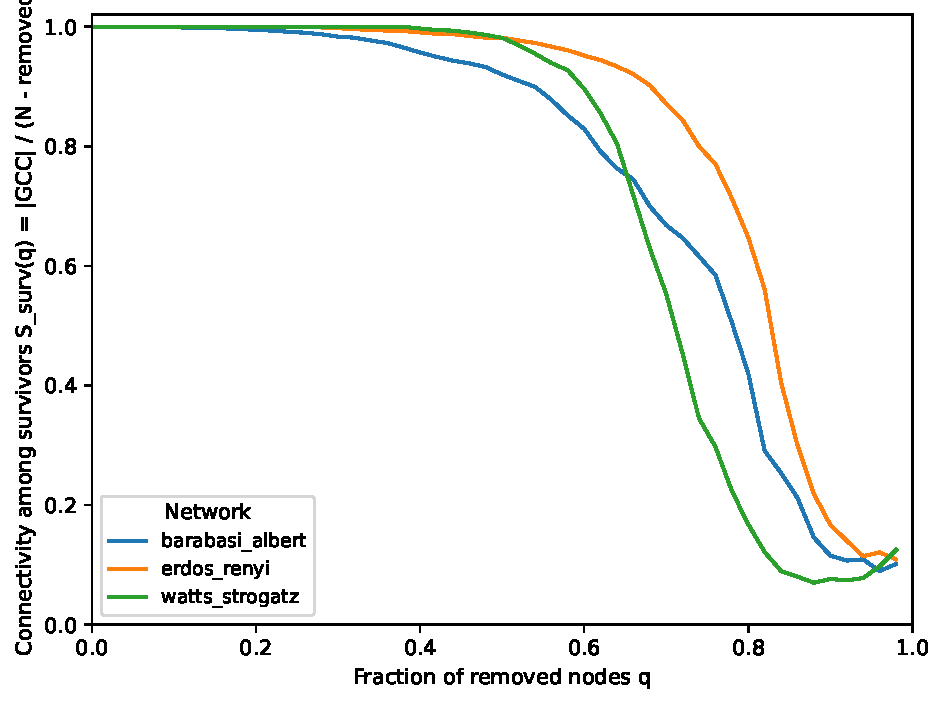
\includegraphics[width=0.9\textwidth]{figures/abb5_random_failures_survivors.pdf}
  \caption{Konnektivität der verbleibenden Knoten unter zufälligen
  Knotenausfällen. Dargestellt ist die normierte Größe der größten verbundenen
  Komponente relativ zur Anzahl der verbleibenden Knoten
  $S_{\text{surv}}(q)=|\mathrm{GCC}(q)|/(N-n_{\text{removed}})$.}
  \label{fig:random_failures_survivors}
\end{figure}


\subsection{Robustheit unter gezielten Angriffen}

In diesem Abschnitt wird das Robustheitsverhalten der untersuchten Netzwerke
unter gezielten Angriffen analysiert. Im Gegensatz zu zufälligen Ausfällen
werden hierbei Knoten nicht zufällig, sondern anhand struktureller
Zentralitätsmaße entfernt. Solche Szenarien modellieren bewusste Angriffe auf
kritische Netzkomponenten und stellen eine Worst-Case-Betrachtung der
Netzwerkstabilität dar.\\
Untersucht werden zwei Angriffstypen: gezielte Angriffe auf Basis des
Knotengrads sowie auf Basis der Betweenness-Zentralität. In beiden Fällen werden
Knoten iterativ in absteigender Reihenfolge des jeweiligen Zentralitätsmaßes
entfernt.

\paragraph{Gradbasierte Angriffe}
Abbildung~\ref{fig:targeted_degree} zeigt die Robustheitskurven unter
gradbasierten Angriffen. Die Unterschiede zwischen den Netzwerkmodellen sind in
diesem Szenario besonders deutlich ausgeprägt. Das Barabási--Albert-Netzwerk
reagiert extrem empfindlich auf die gezielte Entfernung hochgradiger Knoten.
Bereits bei kleinen Anteilen entfernter Knoten bricht die größte verbundene
Komponente nahezu vollständig zusammen.\\
Ursächlich hierfür ist die ausgeprägte Hub-Struktur skalenfreier Netzwerke. Die
Entfernung weniger zentraler Knoten führt dazu, dass große Teile des Netzwerks
ihre Anbindung verlieren. Erdős--Rényi- und Watts--Strogatz-Netzwerke zeigen
demgegenüber eine deutlich höhere Robustheit. Aufgrund ihrer homogeneren
Gradverteilungen erfolgt die Fragmentierung hier schrittweise und erst bei
höheren Angriffsstärken.

\begin{figure}[htbp]
  \centering
  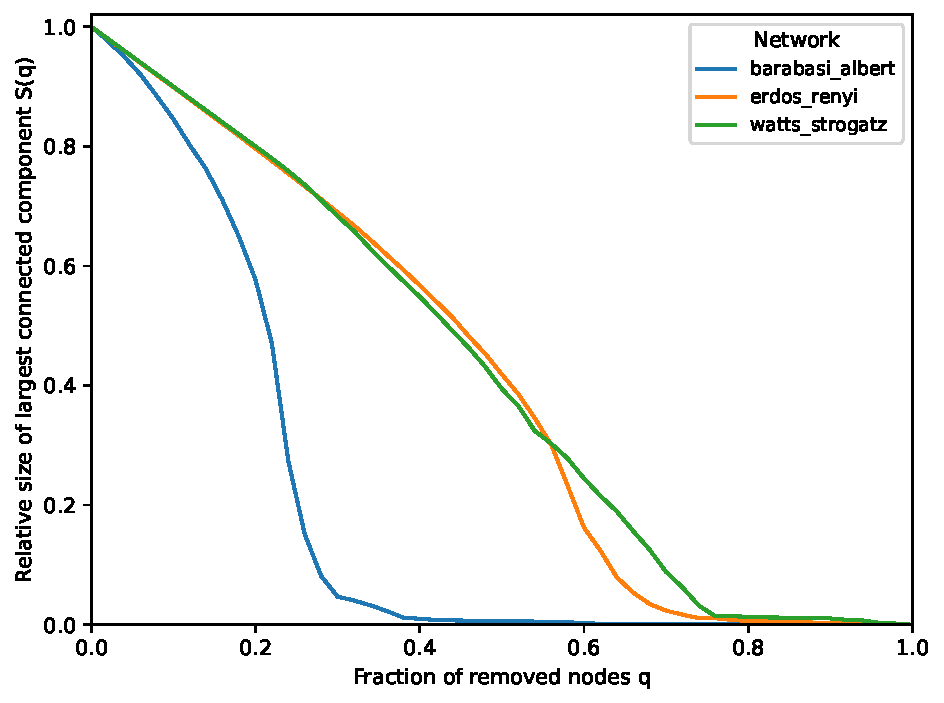
\includegraphics[width=0.9\textwidth]{figures/abb5_targeted_degree_curves.pdf}
  \caption{Robustheitskurven der untersuchten Netzwerkmodelle unter gezielten
  Angriffen auf Basis des Knotengrads.}
  \label{fig:targeted_degree}
\end{figure}

\paragraph{Angriffe nach Betweenness-Zentralität}
Die Auswirkungen gezielter Angriffe auf Basis der Betweenness-Zentralität sind
in Abbildung~\ref{fig:targeted_betweenness} dargestellt. Auch in diesem Szenario
zeigt das Barabási--Albert-Netzwerk eine ausgeprägte Verwundbarkeit. Die
Entfernung weniger Knoten mit hoher Vermittlungsfunktion führt rasch zu einer
Fragmentierung des Netzwerks.\\
Auffällig ist zudem das Verhalten des Watts--Strogatz-Netzwerks. Trotz hoher
lokaler Clusterbildung reagieren diese Netzwerke empfindlich auf
Betweenness-basierte Angriffe, da einzelne Knoten eine zentrale Rolle für die
Verbindung verschiedener Netzwerkbereiche einnehmen. Erdős--Rényi-Netzwerke
weisen auch in diesem Szenario die höchste Robustheit auf, da keine einzelnen
Knoten eine dominierende Vermittlungsfunktion besitzen.

\begin{figure}[htbp]
  \centering
  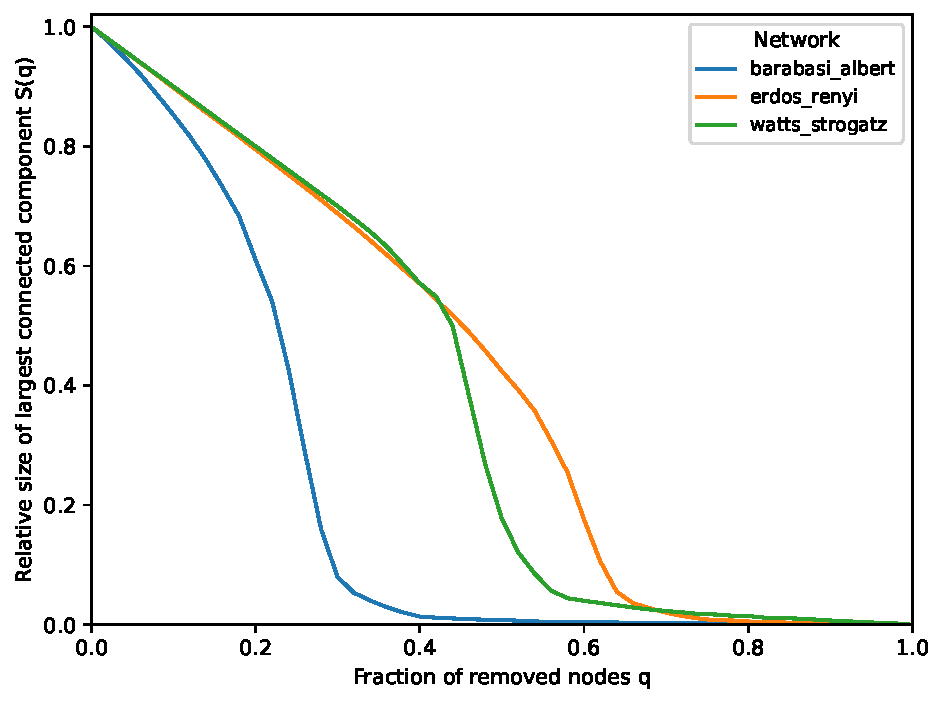
\includegraphics[width=0.9\textwidth]{figures/abb5_targeted_betweenness_curves.pdf}
  \caption{Robustheitskurven der untersuchten Netzwerkmodelle unter gezielten
  Angriffen auf Basis der Betweenness-Zentralität.}
  \label{fig:targeted_betweenness}
\end{figure}

\paragraph{Zusammenfassende Einordnung}
Der Vergleich beider Angriffsszenarien zeigt, dass gezielte Angriffe die
Netzwerkstruktur wesentlich stärker beeinträchtigen als zufällige Ausfälle.
Insbesondere skalenfreie Netzwerke, die unter Random Failures als robust gelten,
erweisen sich unter gezielten Angriffen als hochgradig verwundbar. Die
Simulationen bestätigen damit zentrale theoretische Befunde und verdeutlichen,
dass strukturelle Zentralität ein entscheidender Faktor für die Stabilität
komplexer Netzwerke ist.

\subsection{Zusammenfassender Robustheitsvergleich mittels AUC}

Die bisherigen Abschnitte haben das Robustheitsverhalten der Netzwerke anhand
von Kurvenverläufen illustriert. Für einen kompakten und vergleichbaren
Gesamtüberblick wird im Folgenden die Fläche unter der Robustheitskurve (Area
Under the Curve, AUC) betrachtet. Als zugrunde liegende Größe dient dabei
\[
S(q) = \frac{|\mathrm{GCC}(q)|}{N},
\]
also der relative Anteil der größten verbundenen Komponente in Abhängigkeit vom
entfernten Knotenantteil $q$. Die AUC fasst den gesamten Kurvenverlauf zu einer
einzigen Kennzahl zusammen und erlaubt damit einen direkten quantitativen
Vergleich zwischen Netzwerken und Angriffsszenarien.

\begin{table}[htbp]
\centering
\caption{AUC der Robustheitskurven (größere Werte $\Rightarrow$ höhere Robustheit).}
\label{tab:auc_summary}
\begin{tabular}{lccc}
\hline
Netzwerk & Random Failures & Targeted (Degree) & Targeted (Betweenness) \\
\hline
BA\_n800\_m3 & 0.454 & 0.196 & 0.210 \\
ER\_n800\_p0.01 & 0.476 & 0.408 & 0.407 \\
WS\_n800\_k8\_p0.1 & 0.454 & 0.418 & 0.375 \\
\hline
\end{tabular}
\end{table}


\paragraph{Random Failures}
Unter zufälligen Ausfällen zeigen alle drei synthetischen Netzwerkmodelle
vergleichsweise hohe AUC-Werte. Das Erdős--Rényi-Netzwerk weist mit
$\mathrm{AUC}\approx0{,}48$ die höchste Robustheit auf, gefolgt von
Watts--Strogatz und Barabási--Albert mit nahezu identischen Werten von rund
$0{,}45$. Dieses Ergebnis spiegelt die relativ homogene Struktur der ER-Netze
wider, bei denen zufällige Knotenausfälle die globale Konnektivität erst spät
beeinträchtigen. Gleichzeitig zeigt sich, dass auch skalenfreie Netze bei
ungerichteten Störungen keine besondere strukturelle Schwäche aufweisen.

\paragraph{Gezielte Angriffe nach Knotengrad}
Bei gradbasierten Angriffen tritt ein deutlich anderes Bild auf. Das
Barabási--Albert-Netzwerk bricht frühzeitig zusammen und erreicht mit einer AUC
von etwa $0{,}20$ den mit Abstand niedrigsten Wert. Erdős--Rényi- und
Watts--Strogatz-Netzwerke bleiben dagegen deutlich stabiler
($\mathrm{AUC}\approx0{,}41$). Dieses Ergebnis bestätigt quantitativ die in der
Literatur bekannte hohe Verwundbarkeit skalenfreier Netzwerke gegenüber
gezielten Angriffen auf hochgradige Knoten.

\paragraph{Gezielte Angriffe nach Betweenness}
Auch bei Angriffen auf Knoten mit hoher Betweenness-Zentralität zeigt sich eine
starke Differenz zwischen den Modellen. Das Barabási--Albert-Netzwerk erreicht
erneut nur eine sehr geringe AUC von etwa $0{,}21$, während Erdős--Rényi mit
$\mathrm{AUC}\approx0{,}41$ und Watts--Strogatz mit etwa $0{,}38$ deutlich robuster
bleiben. Im Vergleich zum gradbasierten Angriff fällt der Unterschied zwischen
ER und WS hier stärker ins Gewicht, was auf die Bedeutung vermittelnder
Knotenpositionen in Small-World-Strukturen hindeutet.

\paragraph{Gesamtbewertung}
Die AUC-Auswertung bestätigt die zuvor beobachteten Kurvenverläufe in
kompakter Form. Skalenfreie Netzwerke sind gegenüber zufälligen Ausfällen
vergleichsweise robust, reagieren jedoch extrem empfindlich auf gezielte
Angriffe. Erdős--Rényi- und Watts--Strogatz-Netze zeigen dagegen ein insgesamt
ausgeglicheneres Robustheitsverhalten über alle Szenarien hinweg. Die geringe
Streuung der AUC-Werte über die Wiederholungen hinweg unterstreicht zudem die
Stabilität der beobachteten Effekte.


\end{document}
